\section{Digital Image Correlation} \label{DIC afsnit}
DIC er en optisk metode, der anvender digitale billeder til at måle deformation, bevægelse og tøjning i materialer. DIC fungerer ved at sammenligne billeder taget før, under og efter deformation for at måle forskydninger og udregne tøjninger. Metoden gør det muligt at undersøge deformationer over hele emnet og omkring revner. (\cite{Zaya2023ApplicationReview})

\begin{figure}[H]
    \centering
    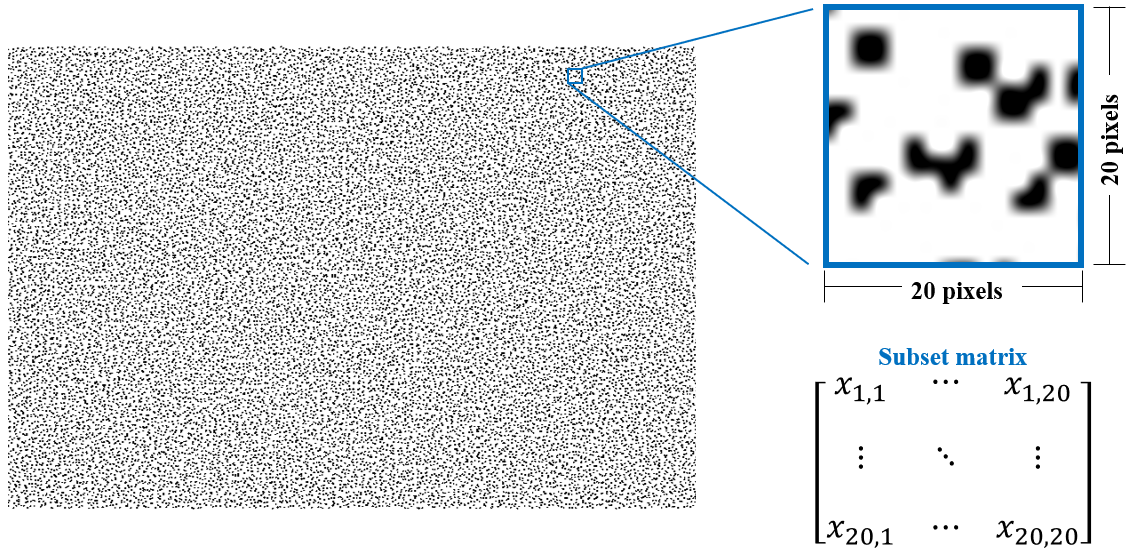
\includegraphics[width=0.85\linewidth]{Sections/2 Problemanalyse/Media/Speckle pattern subset matrix.png}
    \caption{Illustration af speckles pattern, i øverste højre hjørne ses et subset på $20 \times 20 \text{pixels}$ . Det er genereret med software fra Correlated Solutions (\cite{CorrelatedSolutions2025SpeckleInc.})}
    \label{fig:speckle pattern subset}
\end{figure} \plainbreak{-0.5}

DIC starter med et reference billede taget før deformation, eventuelt efterfulgt af billeder taget under deformationsprocessen, samt et billedet efter deformation. Computersoftware bruger forskellen mellem referencebilledet og de efterfølgende billeder, til at finde deformationer, som herefter udregnes til tøjninger i prøven. Softwaren gør dette ved at identificere subsets af pixels (se figur \ref{fig:speckle pattern subset}) i reference billedet, og derefter finder samme deformerede subset på billedet hvor emnet er deformeret. (\cite{Zaya2023ApplicationReview})

DIC benyttes både til undersøgelser af plane emner (2D), samt rumlige emner (3D). I 2D undersøgelser må materialet ikke deformere sig ud af planet, da denne bevægelse ikke kan blive set af kameraet. 3D DIC benytter sig af to eller flere kameraer, og er optimal i situationer, hvor et materiale bevæger sig fra planet til rummet (figur \ref{fig:2D og 3D DIC}).

\begin{figure}[H]
    \centering
    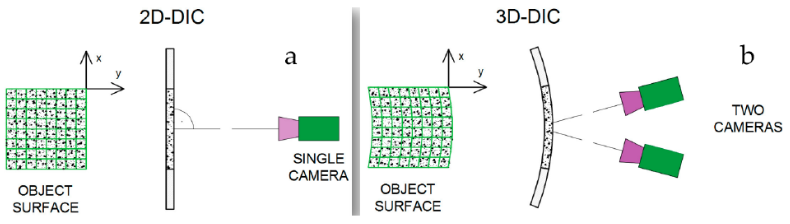
\includegraphics[width=0.9\linewidth]{Sections/2 Problemanalyse/Media/DIC 2D eller 3D.png}
    \caption{Opstilling af 2D og 3D digital image correlation (\cite{Wang2023FiberMonitoring})}
    \label{fig:2D og 3D DIC}
\end{figure} \plainbreak{-0.5}

Opstillingen med flere kameraer giver mulighed for, at tage flere billeder fra forskellige vinkler, og ved hjælp af stereo triangulering, danne en 3D model af objektet. (\cite{Byrne2020DigitalSoftware})


Speckle patterns opdeles i denne rapport i to dele, mikro- og makroskala. I denne rapport defineres mikroskala som den størrelse, der ikke kan opfanges med det blotte øje, og makroskala er den størrelse, der kan fanges med det blotte øje. Der vælges at arbejde i makroskala, med prikker ned til \SI{0,1}{mm} i diameter, fordi det vurderes, at være realistisk at lave speckle patterns i en størrelsesorden man kan se, og ikke mindre.


%Vinklen mellem to kameraer og objektet kaldes stereo vinklen. Denne vinkel kan justeres afhængig af ønsket resultat. Hvis man ønsker større undersøgelse rettet mod et plan, kan vinklen mindskes, og til en rumlig undersøgelse med bevægelse ud af planet, kan vinklen øges. Den optimale vinkel for 3D DIC er mellem 15\degree og 35\degree. (\cite{Bigger2018ACorrelation}) 



\subsection{Alternative målemetoder}
Alternativerne til DIC er primært strain gauges og ekstensometre. Generelt kan de betegnes som spotmålere, det vil sige de måler over et begrænset område, tilgengæld giver de mere nøjagtige målinger end DIC.

\begin{figure}[H]
    \centering
    \begin{subfigure}{0.48\textwidth}
        \centering
        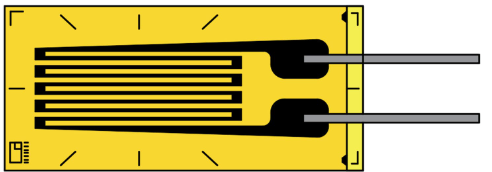
\includegraphics[width=0.8\linewidth]{Sections/2 Problemanalyse/Media/strain gauge.png}
        \caption{Lineær strain gauge der ikke er monteret \parencite{IndustrialQuickSearch2025PrinciplesGauges}}
        \label{fig:straingauge}
    \end{subfigure}
    \begin{subfigure}{0.48\textwidth}
        \centering
        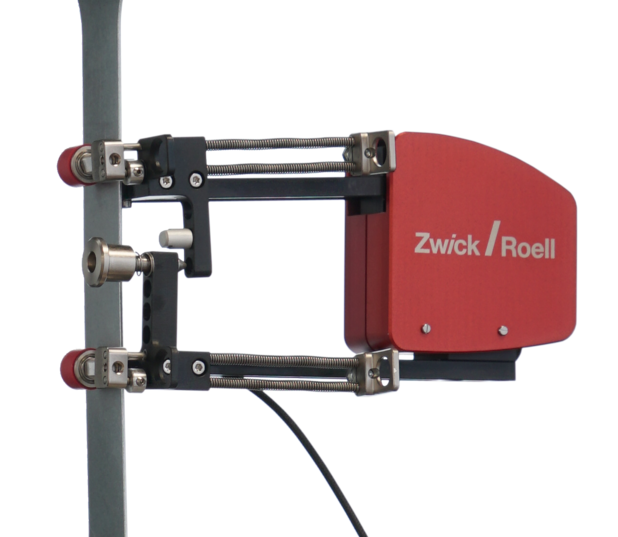
\includegraphics[width=0.7\linewidth]{Sections/2 Problemanalyse/Media/ekstensometer.png}
        \caption{Clip-On ekstensometer monteret \parencite{ZwickRoellExtensometers}}
        \label{fig:ekstensometer}
    \end{subfigure}
    \caption{}
    \label{alternativertildic}
\end{figure} \plainbreak{-0.5}

\textbf{Strain gauges} består af en tynd metalstribe, typisk i zigzaggede parallelle linjer (se figur \ref{fig:straingauge}), på et fleksibelt, isolerende materiale med en form for klistrende underside. Tøjningen findes ved måling af ændringen i modstand, jo mere den deformeres jo højere vil modstanden blive. 

\textbf{Ekstensometre} måler ændringen i afstanden mellem dens to arme, se figur \ref{fig:ekstensometer}. Ekstensiometre kommer i flere varianter der afhænger af,  hvordan armene påsættes emnet.


 

%Siden sin begyndelse i slut 1900-tallet, har DIC gennem årene udviklet sig, og blevet benyttet til en række af forskellige materialeundersøgelser og er blevet til en populær eksperimentel metode blandt andet grundet kosteffektivitet. Materialeundersøgelser som DIC har været igennem inkluderer metaller, polymerer, kompositter, samt biologiske materialer. Disse undersøgelser finder sted på både mikro- og makroskopisk skala, fra millimeter til flere meter. Herved har man også fundet materialer, som ikke er egnet til DIC grundet specifikke faktorer. Nogle af disse inkluderer: Gennemsigtige, bløde eller reflekterende materialer. Løsninger på disse lyder på overfladebelægning af gennemsigtig materiale, benytte speckles af matsort på reflekterende overflader. På bløde materialer er det mere besværligt, men et kamera med en høj rate af billeder i sekundet skal anvendes, grundet skrøbelighed og hurtig deformation. (\cite{Dong2017ACorrelation}; \cite{Bigger2018ACorrelation})